%%% future-work.tex: -*- LaTeX -*-  DESCRIPTIVE TEXT.
%%% 
%%% Copyright (c) 2017 Brian J. Fox & Orchid Labs, Inc.
%%% Author: Brian J. Fox (bfox@meshlabs.org)
%%% Author: A truckload of others
%%% Birthdate: Tue Oct 10 12:09:40 2017.

The items in this section fall into two categories: nice-to-haves, and features we are internally conflicted about releasing to the public. We believe this is conflictedness is universal -- although almost everyone has favorite examples of power being used for oppression, there are also countless examples of power being used for good. Protocols like \Orchid{} have no judgement of their own, and so cannot tell if they are routing traffic for a freedom fighter or a terrorist, villain or hero.

\subsection{Proof of Space}
\label{future:proof-of-space}

As mentioned in Section \ref{medallions}, we are very interested in
exploring alternative proof types. This is an important issue both
because of the environmental impact of proof-of-work systems, and
because our current proof-of-work algorithm requires full blown
computers to act as network routers.

We are excited to explore the possibility of using disk space to be
the scarce resource at the core of our security, which might allow old
phones or similar hardware to profitably participate in the \Orchid{}
network.

\subsection{Protecting Content Hosts}
\label{subsec:protocol-extentions}

Many prior approaches (Section \ref{sec:prior-work}) discovered that content hosts sought similar protections as web users. We are internally conflicted on this point, as we do believe there is content which it is in the public interest not to have freely distributed (information related to the manufacture of nuclear weapons for example). However, should unforseen circumstances demand it, \Orchid{} could be extended to support such ``unrestricted, unsurveilled Hosts'' as seen in the following diagram:

\begin{figure}[htbp]
  \centering
  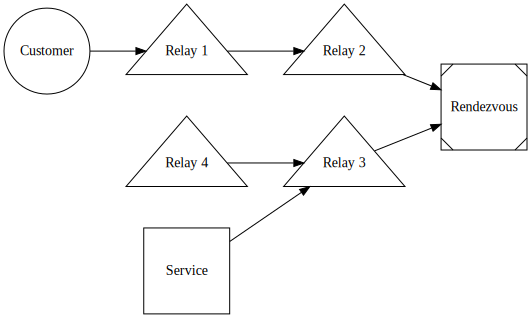
\includegraphics[width = 300pt]{sttRttc}
  \caption{A rendezvous node acting as a relay between a Service and a Customer}
\end{figure}

\subsection{Securing Ethereum Traffic}
\label{securing-eth}

As discussed in our section on firewall avoidance (Section \ref{sec:evasion}),
the Ethereum network traffic of clients is likely to be the weak
link. Because all nodes must maintain this information, use of the
\Orchid{} protocol to distribute Ethereum information seems like a
natural fit.

Unfortunately, relying on those you are paying for information about
payments leads to tricky issues. We hope to add this in the near
future, but will not be including it in our initial release.

\subsection{\Orchid{} as a Platform}

Although we anticipate that design of the core system will take up
much of our time for the immediate future, we are very interested in
the possibility that adding features to support the following use
cases may drastically increase the amount of bandwidth routed through
the \Orchid{} Network.

\begin{enumerate}
\item APIs for websites to directly interface to the network, and
  incorporate tokens into their service.
\item On-Network file storage and static website hosting.
\item File Sharing.
\item Email/Messaging service.
\item An arbitration/moderation service.
\end{enumerate}

%% The issue with modern networking from an surveillance perspective is that it is fundamentally about connections between computers. So long as the model is that a user's computer connects to a specific webserver to access a website, Orchid may be as good as possible. However, if we

